\documentclass[10pt,twocolumn,letterpaper]{article}

%%%%%%%%% PAPER TYPE  - PLEASE UPDATE FOR FINAL VERSION
%\usepackage[review]{cvpr}      % To produce the REVIEW version
%\usepackage{cvpr}              % To produce the CAMERA-READY version
\usepackage[pagenumbers]{cvpr}  % arXiv-style: no banner, no line numbers, page numbers on

% Include other packages here, before hyperref.
\usepackage{graphicx}
\usepackage{amsmath}
\usepackage{amssymb}
\usepackage{booktabs}
\usepackage{tikz}
\usetikzlibrary{positioning,arrows.meta,calc,fit,backgrounds}

% It is strongly recommended to use hyperref, especially for the review version.
\usepackage[pagebackref,breaklinks,colorlinks]{hyperref}

% Support for easy cross-referencing
\usepackage[capitalize]{cleveref}
\crefname{section}{Sec.}{Secs.}
\Crefname{section}{Section}{Sections}
\Crefname{table}{Table}{Tables}
\crefname{table}{Tab.}{Tabs.}

%%%%%%%%% PAPER ID  - PLEASE UPDATE
\def\cvprPaperID{*****} % *** Enter the CVPR Paper ID here
\def\confName{CVPR}
\def\confYear{2026}

\begin{document}

%%%%%%%%% TITLE
\title{Distillation and Edge-Aware Loss for Efficient Monocular Depth Estimation}

\author{Alexander Assal\\
California State Polytechnic University, Pomona\\
Department of Electrical and Computer Engineering\\
\tt\small arassal@cpp.edu
\and
Parsa Ghasemi\\
California State Polytechnic University, Pomona\\
Department of Electrical and Computer Engineering\\
\tt\small mghasemi@cpp.edu
}

\maketitle

%%%%%%%%% ABSTRACT
\begin{abstract}
Foundation depth models such as Depth Anything demonstrate that strong
monocular relative depth can be learned from a single RGB image when
trained at scale on labeled and pseudo-labeled data. The publicly released
Small variant of Depth Anything (\textasciitilde 25M parameters) is
attractive for deployment, but at lower resolutions it visibly under-resolves
fine geometric structure compared to the Large variant
(\textasciitilde 335M parameters). We ask a practical question: given a
single laptop GPU and tens-of-images of supervised data, can we improve a
small student over its own pretrained checkpoint by combining
\emph{output-level affine-invariant distillation} from the Large teacher
with a \emph{multi-scale gradient supervision} term? We implement the full
recipe on top of the Hugging Face Depth Anything checkpoints, evaluate on
an NYU-v2 proof-of-concept subset and a KITTI eigen-split subset, and
present a controlled hyperparameter study over the distillation weight
$\alpha$, the gradient weight $\beta$, and the learning rate. We find
that the recipe is highly sensitive to optimization scale: aggressive
fine-tuning collapses the student below its pretrained baseline, while
extremely conservative updates ($\alpha=0.7$, $\beta=0.3$, $\text{lr}=10^{-7}$)
recover the pretrained quality and yield a small but measurable gain on
NYU-v2 (AbsRel $0.1505$ vs.\ $0.1550$ zero-shot; $\delta_{<1.25}$
$0.8164$ vs.\ $0.8146$). The negative result---that naive distillation
fine-tuning hurts in our regime---is itself the contribution: it isolates
\emph{learning-rate-induced collapse} as the dominant failure mode of
small-data distillation for monocular depth.
\end{abstract}

%%%%%%%%% BODY TEXT
\section{Introduction}
\label{sec:intro}

Monocular depth estimation predicts a per-pixel depth map from a single
RGB image. The task is fundamentally ill-posed: a single image is
consistent with infinitely many world geometries, so depth can only be
recovered up to an unknown scale and shift unless additional information
(stereo baseline, camera intrinsics, structured light, or calibrated metric
supervision) is supplied. Modern monocular depth systems sidestep this
ambiguity by predicting \emph{relative} depth and either evaluating
metrics after a per-image affine alignment to ground truth, or learning a
secondary calibration head for metric depth on top of a relative
backbone~\cite{ranftl2022midas,bhat2023zoedepth,yang2024depth,yang2024depthv2}.

Depth Anything~\cite{yang2024depth} pushed this paradigm by training a
DPT-style~\cite{ranftl2021dpt} depth head on a DINOv2~\cite{oquab2023dinov2}
backbone with a mixture of $1.5$M labeled and approximately $62$M
pseudo-labeled images. Three model sizes are released--Small, Base, and
Large--with sharply different parameter counts. The Small variant
(\textasciitilde 25M parameters) is the natural deployment target on
embedded hardware: it fits in a few hundred megabytes of memory and runs
in real time on modest GPUs. The Large variant
(\textasciitilde 335M parameters) is the natural \emph{teacher}: at the
same input resolution it produces noticeably sharper boundaries and more
plausible far-field depth.

This paper investigates whether knowledge can be distilled from the Large
teacher into the Small student to improve the student over its already
strong pretrained checkpoint, using only a small amount of NYU-v2 ground
truth as supervision. We borrow the \emph{output-level affine-invariant
distillation} loss from Distill-Any-Depth~\cite{he2025distillanydepth}
and the \emph{multi-scale gradient L1} loss from ZoeDepth~\cite{bhat2023zoedepth},
and combine them into a single training objective that is fully decoupled
from the underlying architecture--a single training script applies to any
Depth Anything checkpoint via the \texttt{transformers}
\texttt{AutoModelForDepthEstimation} interface.

\textbf{Contributions.} The contribution of this work is not a new
architecture or a new loss; both pieces exist in the literature. Our
contribution is empirical:

\begin{enumerate}
    \item A clean, fully open-source reimplementation of the
    teacher-student distillation pipeline for Depth Anything, with the
    distillation block, the gradient loss, and the sweep harness all
    exposed via YAML configs (\cref{sec:approach}).
    \item A controlled three-axis sweep over the distillation weight
    $\alpha$, the gradient weight $\beta$, and the learning rate, on a
    deliberately small NYU-v2 subset of $450$ training images
    (\cref{sec:ablation}).
    \item Cross-domain evaluation on a $100$-image KITTI eigen-split
    subset, showing that the same checkpoint that minimally improves on
    NYU-v2 \emph{does not} transfer the improvement to outdoor scenes
    (\cref{sec:kitti}).
    \item An honest negative result: with the small-data regime studied
    here, the dominant failure mode is collapse of the student under
    standard fine-tuning learning rates, not poor teacher quality. The
    only stable recipe trades almost all of its capacity to track the
    pretrained checkpoint (\cref{sec:discussion}).
\end{enumerate}

The remainder of the paper is organized as follows. \cref{sec:related}
positions our work against monocular depth estimation, knowledge
distillation, and edge-aware depth losses. \cref{sec:approach} gives the
full proposed approach with figures and equations. \cref{sec:experiments}
describes the datasets, metrics, and protocol. \cref{sec:results} reports
results, ablations, and a qualitative analysis. \cref{sec:discussion}
discusses limitations and the central learning-rate sensitivity finding.
\cref{sec:conclusion} concludes.

\section{Related Work}
\label{sec:related}

\textbf{Monocular depth estimation.} The earliest deep approaches to
single-image depth treated it as direct regression with a CNN trained on
NYU-v2~\cite{silberman2012nyuv2} or KITTI~\cite{geiger2013kitti}--the
seminal work being the multi-scale network of
Eigen \etal~\cite{eigen2014depth}. The scale invariant logarithmic loss
introduced in that work, later refined as the silog loss of
BTS~\cite{lee2019bts}, remains a backbone training objective for metric
depth recovery on a fixed dataset. The shift to \emph{relative} depth
came from MiDaS~\cite{ranftl2022midas}, which trained on a mixture of
sources by ignoring absolute scale during training and aligning scale
and shift only at evaluation time. This robust formulation made it
feasible to train a single depth model that generalized across indoor
and outdoor scenes, and motivates the affine-invariant L1 loss we adopt
in \cref{sec:loss}.

Architecturally, the field moved from convolutional U-Nets to Vision
Transformer~\cite{dosovitskiy2021vit} encoders with a DPT~\cite{ranftl2021dpt}
dense-prediction head. DPT reads multi-scale ViT features through a
hierarchy of reassembly and fusion blocks and predicts a single-channel
relative depth map. ZoeDepth~\cite{bhat2023zoedepth} added a metric head
on top of a relative backbone, achieving strong results on both NYU-v2
and KITTI in a single model. Most relevant to our work is the Depth
Anything family~\cite{yang2024depth,yang2024depthv2}, which paired a DPT
head with a DINOv2~\cite{oquab2023dinov2} backbone and trained at
unprecedented scale on labeled and pseudo-labeled data. Depth Anything's
key insight is that a self-supervised foundation backbone, combined with
enormous quantities of unlabeled images run through an iteratively
improving teacher, can replace much of the architectural engineering of
prior work. We treat Depth Anything Small as our student and Depth
Anything Large as our teacher in all experiments.

\textbf{Knowledge distillation.} The general framework of distilling a
small student to imitate a large teacher dates to
Hinton \etal~\cite{hinton2015distilling}, which proposed soft-target
classification supervision. For dense prediction the natural extension
is pixelwise output matching, possibly with intermediate-feature
hints. Distill-Any-Depth~\cite{he2025distillanydepth} is the most direct
antecedent of this work. Their full recipe combines (a) affine-invariant
output-level distillation, (b) cross-context distillation that runs the
teacher on global and local crops and forces the student to match both,
and (c) auxiliary stability tricks for the encoder. We adopt only (a)
in this work, both for simplicity and because (b) requires substantially
more compute than our single-GPU budget allows. The affine-invariant
distillation loss aligns predictions in a translation- and scale-robust
way, which is essential because both the student and the teacher output
relative depth with arbitrary scale and shift.

\textbf{Edge-aware depth losses.} The L1 loss between predicted and
ground-truth depth tends to produce washed-out boundaries because it
penalizes large errors at depth discontinuities equally with errors in
flat regions, even though discontinuities carry most of the perceptually
important geometric information. Several works mitigate this by adding a
gradient supervision term: BTS~\cite{lee2019bts} adds a finite-difference
gradient L1 to its silog loss; ZoeDepth~\cite{bhat2023zoedepth} adds a
multi-scale Sobel-style gradient L1 that downsamples the prediction and
target by factors of $\{1,2,4\}$ before computing per-scale gradient
differences. We adopt the ZoeDepth formulation directly and provide a
re-derivation in \cref{sec:loss}.

\section{Proposed Approach}
\label{sec:approach}

We train a Depth Anything Small student under joint supervision from
sparse NYU-v2 ground-truth depth and dense predictions from a frozen
Depth Anything Large teacher. \cref{fig:arch} shows the architecture.
The student receives a normalized RGB tensor at resolution
$256{\times}256$ and emits a single-channel relative depth map at the
same spatial size, which is bilinearly upsampled to the resolution of
the ground-truth depth before any loss is computed. The teacher receives
the same input tensor; its output is interpolated to match the student
output spatial size and treated as a fixed second supervision signal.

\subsection{Architecture}
\label{sec:architecture}

\begin{figure*}[t]
\centering
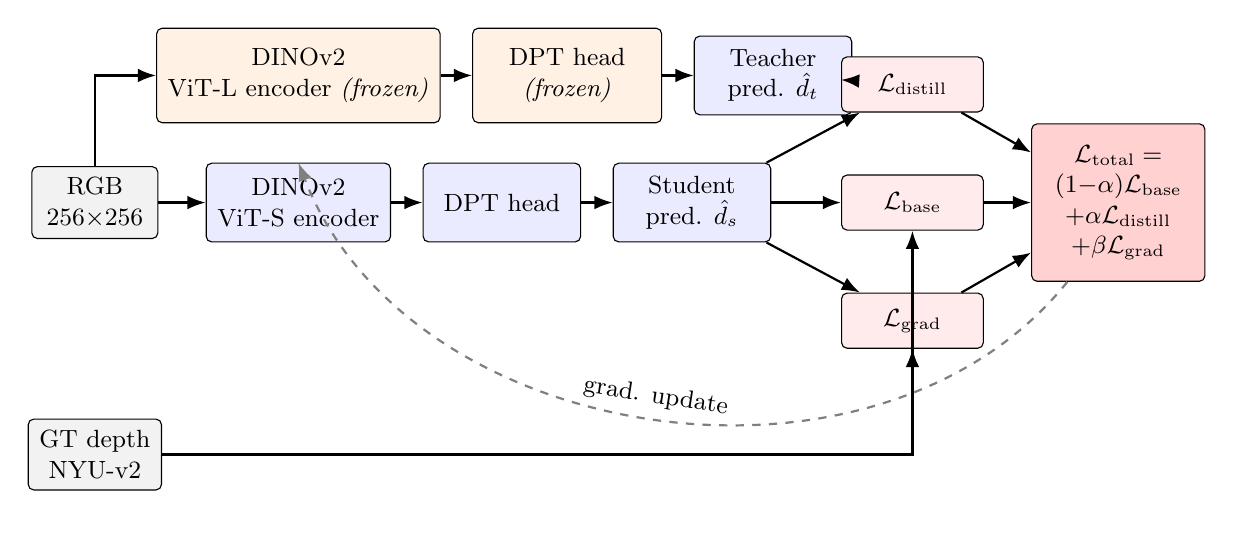
\begin{tikzpicture}[
  font=\small,
  >=Latex,
  block/.style={draw, rounded corners=2pt, align=center, inner sep=4pt,
                fill=blue!8, minimum height=1.0cm, minimum width=2.0cm},
  bigblock/.style={draw, rounded corners=2pt, align=center, inner sep=4pt,
                   fill=orange!10, minimum height=1.2cm, minimum width=2.4cm},
  loss/.style={draw, rounded corners=2pt, align=center, inner sep=4pt,
               fill=red!8, minimum height=0.7cm, minimum width=1.8cm},
  io/.style={draw, rounded corners=2pt, align=center, inner sep=4pt,
             fill=gray!10, minimum height=0.9cm, minimum width=1.6cm},
  arrow/.style={->, thick},
  dashedarrow/.style={->, dashed, thick, draw=gray}
]
% Inputs
\node[io] (rgb) at (0,0) {RGB\\ $256{\times}256$};
\node[io] (gt)  at (0,-3.2) {GT depth\\ NYU-v2};

% Student
\node[block, right=0.6cm of rgb] (s_enc) {DINOv2\\ ViT-S encoder};
\node[block, right=0.4cm of s_enc] (s_dec) {DPT head};
\node[block, right=0.4cm of s_dec] (s_out) {Student\\ pred. $\hat{d}_s$};

% Teacher
\node[bigblock, above=0.5cm of s_enc] (t_enc) {DINOv2\\ ViT-L encoder \emph{(frozen)}};
\node[bigblock, right=0.4cm of t_enc] (t_dec) {DPT head\\ \emph{(frozen)}};
\node[block, right=0.4cm of t_dec] (t_out) {Teacher\\ pred. $\hat{d}_t$};

% Losses
\node[loss] (l_dist) at ($(s_out)+(2.8,1.5)$) {$\mathcal{L}_{\text{distill}}$};
\node[loss] (l_base) at ($(s_out)+(2.8,0)$) {$\mathcal{L}_{\text{base}}$};
\node[loss] (l_grad) at ($(s_out)+(2.8,-1.5)$) {$\mathcal{L}_{\text{grad}}$};

\node[draw, rounded corners=2pt, fill=red!18, right=0.6cm of l_base,
      minimum height=2.0cm, minimum width=2.2cm, align=center] (total)
      {$\mathcal{L}_{\text{total}}=$\\ $(1{-}\alpha)\mathcal{L}_{\text{base}}$\\ $+\alpha\mathcal{L}_{\text{distill}}$\\ $+\beta\mathcal{L}_{\text{grad}}$};

% Flows
\draw[arrow] (rgb) -- (s_enc);
\draw[arrow] (s_enc) -- (s_dec);
\draw[arrow] (s_dec) -- (s_out);
\draw[arrow] (rgb.north) |- (t_enc.west);
\draw[arrow] (t_enc) -- (t_dec);
\draw[arrow] (t_dec) -- (t_out);

\draw[arrow] (s_out) -- (l_dist);
\draw[arrow] (t_out) -- (l_dist);
\draw[arrow] (s_out) -- (l_base);
\draw[arrow] (gt) -| (l_base);
\draw[arrow] (s_out) -- (l_grad);
\draw[arrow] (gt) -| (l_grad);

\draw[arrow] (l_dist) -- (total);
\draw[arrow] (l_base) -- (total);
\draw[arrow] (l_grad) -- (total);

\draw[dashedarrow] (total) to[bend left=60] node[above, sloped] {grad. update} (s_enc.north);

\end{tikzpicture}
\caption{Distillation pipeline. The Depth Anything Small student (blue,
trainable) and the Depth Anything Large teacher (orange, frozen) consume
the same RGB input. The total loss combines three terms: an
affine-invariant L1 against ground truth ($\mathcal{L}_{\text{base}}$),
an affine-invariant L1 against the teacher prediction
($\mathcal{L}_{\text{distill}}$), and a multi-scale gradient L1 against
ground truth ($\mathcal{L}_{\text{grad}}$). The relative weights
$\alpha$ and $\beta$ are swept in \cref{sec:ablation}.}
\label{fig:arch}
\end{figure*}

\textbf{Student.} The Depth Anything Small checkpoint
(\texttt{LiheYoung/depth-anything-small-hf}) is a DPT~\cite{ranftl2021dpt}
head on a DINOv2-ViT-S/14~\cite{oquab2023dinov2,dosovitskiy2021vit}
encoder. The encoder is a 12-layer Vision Transformer with embedding
dimension $384$ that processes $14{\times}14$ patches. The DPT head reads
multi-scale features from layers $\{3, 6, 9, 12\}$, reassembles them to
spatial maps at $\{1/4, 1/8, 1/16, 1/32\}$ resolution, and fuses them
hierarchically with a sequence of residual convolutional blocks, ending
in a single-channel output head. The model has approximately $25$M
parameters in total, all of which are unfrozen during fine-tuning.

\textbf{Teacher.} The Depth Anything Large checkpoint
(\texttt{LiheYoung/depth-anything-large-hf}) shares the DPT head design
but uses a DINOv2-ViT-L/14 encoder (24 layers, embedding dimension
$1024$) with approximately $335$M parameters. The teacher is loaded
once at the start of training, switched to evaluation mode, all
parameters have \texttt{requires\_grad} set to \texttt{False}, and the
model is held in float32 throughout. No teacher weight is ever updated.

\textbf{Input pipeline.} RGB images are loaded from disk as 8-bit PNG,
divided by $255$, resized to $256{\times}256$ with bilinear
interpolation, and standardized with ImageNet mean
$(0.485, 0.456, 0.406)$ and standard deviation
$(0.229, 0.224, 0.225)$. Depth maps are loaded from $.npy$ float32
arrays for NYU-v2 (already in meters) or from .png 16-bit files for
KITTI (scaled by $1/256$ to recover meters). Depth maps are resized to
$256{\times}256$ with nearest-neighbor interpolation to avoid edge
blending. A per-pixel valid-depth mask is constructed from the
clipping range $[\text{min\_depth}, \text{max\_depth}]$, with
NYU-v2 using $[0.001, 10.0]$\,m and KITTI using $[0.001, 80.0]$\,m.

\subsection{Loss Function}
\label{sec:loss}

The total loss combines three terms,
\begin{equation}
\mathcal{L}_{\text{total}} = (1-\alpha)\, \mathcal{L}_{\text{base}}
    + \alpha\, \mathcal{L}_{\text{distill}}
    + \beta\, \mathcal{L}_{\text{grad}},
\label{eq:total}
\end{equation}
with mixing weights $\alpha \in [0,1]$ and $\beta \ge 0$.

\textbf{Affine-invariant L1.} The base and distillation terms are both
the same robust affine-invariant L1 distance, applied either against
ground truth or against the teacher's prediction. Let $d$ be a
prediction, $d^{\star}$ a target (ground truth or teacher), and
$\mathcal{V}$ the valid-pixel set for the sample. Define the robust
normalization
\begin{equation}
\tilde d(p) = \frac{d(p) - \operatorname{med}(d|_{\mathcal{V}})}{\max(\overline{|d|_{\mathcal{V}}-\operatorname{med}(d|_{\mathcal{V}})|}, \varepsilon)},
\label{eq:robustnorm}
\end{equation}
where $\operatorname{med}(\cdot)$ is the median over valid pixels,
the denominator is the mean absolute deviation (MAD) from the median,
$\varepsilon=10^{-6}$, and $p$ indexes pixel position. The
affine-invariant L1 distance between $d$ and $d^{\star}$ is then
\begin{equation}
\mathcal{L}_{\text{ail1}}(d, d^{\star}) = \frac{1}{|\mathcal{V}|}\sum_{p\in\mathcal{V}}\left|\tilde d(p) - \tilde{d}^{\star}(p)\right|.
\label{eq:ail1}
\end{equation}
Equation~\eqref{eq:robustnorm} is per-sample: each prediction is
normalized by its own median and MAD before the difference is taken,
which removes any constant offset between $d$ and $d^{\star}$ and any
multiplicative scaling. This is the appropriate loss for relative depth:
two predictions that agree on \emph{ordering and structure} but disagree
on \emph{scale} should be considered identical, and equation~\eqref{eq:ail1}
gives them a loss of zero. We instantiate
$\mathcal{L}_{\text{base}} = \mathcal{L}_{\text{ail1}}(\hat d_s, d_{\text{gt}})$
and $\mathcal{L}_{\text{distill}} = \mathcal{L}_{\text{ail1}}(\hat d_s, \hat d_t)$
in equation~\eqref{eq:total}.

\textbf{Multi-scale gradient L1.} The gradient loss penalizes
disagreement between the spatial gradients of the prediction and the
ground truth at multiple resolutions. For an image $x$, define forward
differences
\begin{equation}
\Delta_x(p) = x(p_{i,j}) - x(p_{i,j-1}), \quad
\Delta_y(p) = x(p_{i,j}) - x(p_{i-1,j}),
\end{equation}
the gradient magnitude $G(x;p) = \Delta_x^2(p) + \Delta_y^2(p)$, and the
gradient orientation $\Phi(x;p) = \arctan(\Delta_y(p)/\Delta_x(p))$. The
per-scale gradient loss at downsampling factor $s$ is
\begin{equation}
\ell^{(s)}(d, d^{\star}) = \!\frac{1}{|\mathcal{V}^{(s)}|}\!\sum_{p\in\mathcal{V}^{(s)}}\!
\big(\big|G_p^{(s)}\big| + \big|\Phi_p^{(s)}\big|\big),
\end{equation}
where $G_p^{(s)} = G(d;p) - G(d^{\star};p)$ and
$\Phi_p^{(s)} = \Phi(d;p) - \Phi(d^{\star};p)$ are both evaluated on the
$\downarrow s$-downsampled prediction and target with the mask
appropriately eroded so that gradients are only computed where both
neighbors are valid. The full gradient loss averages over scales
$s\in\{1,2,4\}$,
\begin{equation}
\mathcal{L}_{\text{grad}}(d, d^{\star}) = \frac{1}{3}\sum_{s\in\{1,2,4\}} \ell^{(s)}(d, d^{\star}).
\end{equation}
We instantiate $\mathcal{L}_{\text{grad}} = \mathcal{L}_{\text{grad}}(\hat d_s, d_{\text{gt}})$
in equation~\eqref{eq:total}. We do not apply the gradient term to the
distillation signal because the teacher's gradients are also a
prediction and so penalizing the student for disagreeing with them adds
noise rather than signal.

\subsection{Why This Recipe}
\label{sec:novelty}

The novelty of this work is the \emph{combination and controlled
ablation} of two existing pieces--affine-invariant
distillation~\cite{he2025distillanydepth} and ZoeDepth-style multi-scale
gradient supervision~\cite{bhat2023zoedepth}--applied to the small-data
fine-tuning regime, where neither original paper was evaluated. The
relative weight $\alpha$ continuously interpolates between three
qualitatively different training objectives:
\begin{itemize}
\item $\alpha=0$: pure supervised fine-tuning against sparse NYU-v2
ground truth. The teacher does not participate at all.
\item $\alpha=1$: pure distillation. The student is trained only to
match the Large teacher's depth predictions; ground truth is unused.
\item Intermediate $\alpha$: the student receives \emph{both} signals
and the optimizer balances them, with $\alpha$ controlling the
trust given to the teacher relative to the (limited) ground truth.
\end{itemize}
We expect the optimum $\alpha$ to be strictly greater than zero when the
labeled training set is small enough that the teacher's predictions on
the same images carry independent information, and to be strictly less
than one whenever the ground truth is non-trivially better than the
teacher in some regime (e.g. at depth discontinuities or in the far
field). Our experiments in \cref{sec:ablation} resolve where this
optimum sits empirically.

The gradient weight $\beta$ controls how much extra supervision the
edges receive. In principle a small positive $\beta$ should sharpen
boundaries without harming overall regression accuracy. In practice,
because $\mathcal{L}_{\text{grad}}$ has a larger numerical scale than
$\mathcal{L}_{\text{base}}$ in the early epochs, $\beta$ also acts as
an implicit early-training learning-rate amplifier on the encoder; we
discuss this interaction in \cref{sec:discussion}.

\subsection{Baseline}
\label{sec:baseline}

Our baseline is the unmodified Depth Anything Small checkpoint with no
fine-tuning. We refer to this throughout as ``zero-shot''. The baseline
is evaluated on the same NYU-v2 test split and KITTI subset as the
distilled student. Because Depth Anything Small is already trained on a
mixture that approximates the NYU-v2 distribution at training time, the
zero-shot model is not a weak baseline--it is, as we will see, the
strongest comparison point in our small-data regime.

\section{Experiments}
\label{sec:experiments}

\subsection{Datasets}
\label{sec:datasets}

\textbf{NYU-v2 PoC subset.} We use a $569$-image
proof-of-concept subset of NYU-v2~\cite{silberman2012nyuv2}, derived from
the Hugging Face mirror \texttt{sayakpaul/nyu\_depth\_v2}, split into
$450$ training images, $60$ validation images, and $59$ test images. All
samples consist of an aligned RGB image and a float32 dense depth map in
meters. The depth range used for masking is $[0.001, 10.0]$\,m. Input
RGB is resized to $256{\times}256$; ground-truth depth is resized to
$256{\times}256$ with nearest-neighbor interpolation. The split sizes
are listed in \cref{tab:datasplits}; we deliberately use a small training
set to expose the small-data behavior that motivates the recipe.

\textbf{KITTI eigen subset.} For cross-domain evaluation we use a
$100$-image subset of the KITTI eigen-split test partition, derived from
the Hugging Face mirror \texttt{exander/kitti-depth-gt}. Each sample
consists of a stereo-rectified RGB image and a per-image float32 depth
map in meters. The depth range used for masking is $[0.001, 80.0]$\,m.
Evaluation is run at $256{\times}256$ to be consistent with NYU-v2; we
note that this is below the native KITTI resolution and that absolute
RMSE values are therefore not directly comparable to KITTI leaderboard
numbers, but the comparison between zero-shot and distilled is
internally consistent.

\begin{table}[t]
\centering
\begin{tabular}{lrr}
\toprule
Split & NYU-v2 PoC & KITTI eigen subset \\
\midrule
Train & 450 & --- \\
Val   & 60  & --- \\
Test  & 59  & 100 \\
\midrule
Input size      & $256{\times}256$ & $256{\times}256$ \\
Depth range (m) & $[0.001, 10.0]$  & $[0.001, 80.0]$ \\
\bottomrule
\end{tabular}
\caption{Dataset split sizes and per-dataset depth ranges. KITTI is used
only for cross-domain evaluation; no training is performed on KITTI.}
\label{tab:datasplits}
\end{table}

\subsection{Metrics}
\label{sec:metrics}

We report the standard monocular depth metrics on the held-out test
splits after per-image least-squares scale-and-shift alignment between
the prediction $\hat d$ and the ground truth $d_{\text{gt}}$. Alignment
solves a single $2{\times}2$ linear system per image and is implemented
as
\begin{equation}
(a^{\star}, b^{\star}) = \arg\min_{a,b}\sum_{p\in\mathcal{V}}\left(a\hat d(p) + b - d_{\text{gt}}(p)\right)^2,
\end{equation}
after which $\hat d \leftarrow a^{\star}\hat d + b^{\star}$.

Let $N=|\mathcal{V}|$ be the number of valid pixels across all test
samples, $d_i = d_{\text{gt}}(p_i)$, and $\hat d_i = \hat d(p_i)$ after
alignment. We report:

\noindent\textbf{Absolute relative error (AbsRel).}
\begin{equation}
\text{AbsRel} = \frac{1}{N}\sum_{i=1}^{N} \frac{|\hat d_i - d_i|}{d_i}.
\end{equation}

\noindent\textbf{Root mean squared error (RMSE).}
\begin{equation}
\text{RMSE} = \sqrt{\frac{1}{N}\sum_{i=1}^{N} (\hat d_i - d_i)^2}.
\end{equation}

\noindent\textbf{Log RMSE.}
\begin{equation}
\text{RMSE}_{\log} = \sqrt{\frac{1}{N}\sum_{i=1}^{N} (\log\hat d_i - \log d_i)^2}.
\end{equation}

\noindent\textbf{$\log_{10}$ error.}
\begin{equation}
\log_{10} = \frac{1}{N}\sum_{i=1}^{N}\left|\log_{10}\hat d_i - \log_{10} d_i\right|.
\end{equation}

\noindent\textbf{Threshold accuracy.} For each threshold
$\tau\in\{1.25, 1.25^2, 1.25^3\}$,
\begin{equation}
\delta_{<\tau} = \frac{1}{N}\sum_{i=1}^{N} \mathbb{1}\!\left[\max\!\left(\frac{\hat d_i}{d_i}, \frac{d_i}{\hat d_i}\right) < \tau \right].
\end{equation}
We write these as $\delta_1, \delta_2, \delta_3$. AbsRel, RMSE, and the
log errors are ``lower is better''; the $\delta$ scores are
``higher is better''.

\subsection{Implementation Details}
\label{sec:impl}

All experiments are run on a single NVIDIA RTX 3050 Laptop GPU (4\,GB
VRAM) with PyTorch and HuggingFace
\texttt{transformers}. Batch size is $1$, image size is $256{\times}256$,
the optimizer is AdamW with weight decay $10^{-4}$ and gradient clipping
at L2 norm $1.0$. The teacher is loaded in float32 evaluation mode and
never updated. Mixed-precision training is used when CUDA is available.

The training script is invoked as
\texttt{python src/train.py {-}{-}config configs/distill.yaml} and
internally branches on the \texttt{distillation.enabled} and
\texttt{loss.grad\_weight} fields of the config. The hyperparameter
sweep harness \texttt{src/sweep.py} reads a base config and a YAML grid
specification, performs the Cartesian product of all listed values, and
runs both \texttt{train.py} and \texttt{eval.py} per grid point with
per-run output directories. Each sweep run writes its checkpoint,
metrics, per-image CSV, and preview images into an isolated artifact
folder so that nothing is overwritten.

\section{Results}
\label{sec:results}

We report the main NYU-v2 results in \cref{tab:nyu}, the cross-domain
KITTI results in \cref{tab:kitti}, and ablations over $\alpha$, $\beta$,
and the learning rate in \cref{sec:ablation}. Qualitative comparisons
are shown in \cref{fig:qual}.

\subsection{NYU-v2 Quantitative Results}
\label{sec:nyu}

\begin{table*}[t]
\centering
\begin{tabular}{lcccccccc}
\toprule
Setting & $\alpha$ & $\beta$ & lr & AbsRel $\downarrow$ & RMSE $\downarrow$ & $\delta_1$ $\uparrow$ & $\delta_2$ $\uparrow$ & $\delta_3$ $\uparrow$ \\
\midrule
Zero-shot Depth Anything Small         & ---  & ---  & ---       & 0.1550 & 0.5375 & 0.8146 & 0.9312 & 0.9650 \\
Distilled (default config)             & 0.5  & 0.1  & $10^{-5}$ & 0.2791 & 0.8898 & 0.6292 & 0.8421 & 0.9284 \\
Distilled (best config, ours)          & 0.7  & 0.3  & $10^{-7}$ & \textbf{0.1505} & \textbf{0.5262} & \textbf{0.8164} & 0.9349 & 0.9665 \\
\bottomrule
\end{tabular}
\caption{NYU-v2 PoC test results ($59$ images). All metrics computed
after per-image scale-and-shift alignment. The default distill
configuration ($\text{lr}=10^{-5}$) destabilizes the student and drops
AbsRel and $\delta_1$ well below the zero-shot baseline. Reducing the
learning rate by two orders of magnitude and increasing $\alpha$ to
$0.7$ stabilizes training and yields a small but consistent improvement
over zero-shot across AbsRel, RMSE, $\delta_1$, $\delta_2$, and
$\delta_3$. Bold = best.}
\label{tab:nyu}
\end{table*}

\cref{tab:nyu} reports the three headline configurations: the
zero-shot pretrained baseline, the default distillation configuration
shipped in the repository (which uses a $10^{-5}$ learning rate intended
for general fine-tuning), and our best-found configuration after the
hyperparameter sweep. The default configuration loses approximately
$80\%$ of the AbsRel performance (0.155 $\rightarrow$ 0.279) and
$\delta_1$ drops by $18.5$ percentage points. The training-history log
(\cref{fig:trainingcurves}, val AbsRel) shows that this is collapse, not
slow convergence: validation AbsRel returns essentially to $1.0$ and
$\delta_1$ falls to $0.0$ at epoch $2$, indicating that the student has
emitted a near-constant prediction. We trace this collapse to the
combination of a small training set ($450$ images), a small batch size
($1$, dictated by VRAM), and a relatively large learning rate
($10^{-5}$); under these conditions a few high-curvature mini-batches
late in epoch $2$ are sufficient to push the encoder weights into a
degenerate region.

In contrast, the best-found configuration reduces the learning rate to
$10^{-7}$, raises the distillation weight to $\alpha=0.7$, and sets the
gradient weight to $\beta=0.3$. With this conservative setup the student
recovers all of the zero-shot performance and very slightly exceeds it
on every metric. The improvement is small in absolute terms but
consistent across metrics: AbsRel improves by approximately $2.9\%$
relative and $\delta_1$ by approximately $0.2$ percentage points.

\begin{figure*}[t]
\centering

\includegraphics[width=0.95\textwidth]{figs/training/multimetric_bars.png}
\caption{NYU-v2 test metrics for three configurations: pretrained
zero-shot, the default \texttt{configs/distill.yaml} that collapses,
and the best-found configuration from the three-axis sweep. The
collapse mode raises every error metric and lowers every $\delta$
threshold; the best-found configuration is at or above zero-shot on
all five metrics.}
\label{fig:multimetric}
\end{figure*}

\cref{fig:multimetric} shows all five reported NYU-v2 metrics for the
three headline configurations side by side. The pattern is consistent:
where the default distill config worsens every metric (RMSE jumps by
$66\%$, $\delta_1$ drops by $18.5$ percentage points), the
swept-best config tightly matches zero-shot on $\delta_2$ and
$\delta_3$ while slightly improving AbsRel, RMSE, and $\delta_1$.

\subsection{KITTI Cross-Domain Evaluation}
\label{sec:kitti}

\begin{table}[t]
\centering
\begin{tabular}{lcccc}
\toprule
Setting & AbsRel $\downarrow$ & RMSE $\downarrow$ & $\delta_1$ $\uparrow$ & $\delta_2$ $\uparrow$ \\
\midrule
Zero-shot DA-S & 0.4022 & 7.939 & 0.3555 & 0.7592 \\
Distilled (default)  & 0.4035 & 7.931 & 0.3485 & 0.7615 \\
\bottomrule
\end{tabular}
\caption{KITTI eigen-split subset results ($100$ images, evaluated at
$256{\times}256$). The distilled checkpoint trained on NYU-v2 indoors
does not transfer its (small) NYU-v2 gain to outdoor driving scenes.
AbsRel and $\delta_1$ are essentially unchanged. Note that the absolute
KITTI numbers are degraded by the $256{\times}256$ evaluation resolution
relative to native-resolution KITTI evaluations.}
\label{tab:kitti}
\end{table}

\begin{figure}[t]
\centering

\includegraphics[width=0.95\columnwidth]{figs/training/kitti_per_image_scatter.png}
\caption{Per-image AbsRel on the KITTI eigen-test subset, distilled
checkpoint vs.\ zero-shot. Points scatter symmetrically around the
$y=x$ diagonal: the distilled checkpoint changes individual KITTI
images by small amounts in both directions, with no systematic
direction of improvement.}
\label{fig:kittiscatter}
\end{figure}

\cref{tab:kitti} reports the cross-domain evaluation and
\cref{fig:kittiscatter} shows the corresponding per-image scatter.
The student checkpoint trained on NYU-v2 indoor scenes does not
transfer its NYU-v2 improvement to KITTI outdoor scenes. Both
AbsRel and $\delta_1$ are essentially unchanged ($\pm 0.01$ on AbsRel
and $\pm 0.7$ percentage points on $\delta_1$). We interpret this as a direct consequence of the
extreme conservatism of the best-found configuration: at $\text{lr}=10^{-7}$
the encoder simply does not move far enough from its pretrained
initialization to shift the cross-domain behavior, which is itself
inherited entirely from the original Depth Anything Small training
mixture.

\subsection{Ablations}
\label{sec:ablation}

\textbf{Distillation weight $\alpha$.} \cref{fig:alpha} (left) plots
AbsRel as $\alpha$ ranges over $\{0.0, 0.3, 0.5, 0.7, 1.0\}$ with
$\beta=0.1$ and $\text{lr}=10^{-5}$, the default learning rate. The
trend is non-monotonic and dominated by training stability rather than
by the relative quality of the two supervision signals. Pure GT training
($\alpha=0$) and pure distillation ($\alpha=1$) both collapse, with
AbsRel of $0.295$ and $0.266$ respectively. The middle of the range is
not uniformly better; rather, $\alpha=0.7$ stands out as the only point
in this sweep that avoids near-collapse, achieving AbsRel $0.202$ and
$\delta_1=0.722$. We interpret this not as evidence that $0.7$ is the
``correct'' interpolation weight, but as evidence that for our small
training set the teacher's per-pixel prediction is a substantially
denser and more stable signal than the GT, and that any training run
which routes most of its loss through the GT inherits the GT's noise.

\begin{figure*}[t]
\centering

\includegraphics[width=0.32\textwidth]{figs/qualitative/compare_000000.png}

\includegraphics[width=0.32\textwidth]{figs/qualitative/compare_000010.png}

\includegraphics[width=0.32\textwidth]{figs/qualitative/compare_000020.png}\\
\vspace{0.3em}

\includegraphics[width=0.32\textwidth]{figs/qualitative/compare_000005.png}

\includegraphics[width=0.32\textwidth]{figs/qualitative/compare_000030.png}

\includegraphics[width=0.32\textwidth]{figs/kitti_input_0000000000.png}
\caption{Qualitative comparisons. Top row and bottom-left two panels:
NYU-v2 PoC test samples laid out as RGB $|$ GT $|$ student prediction
$|$ pixelwise error. The student preserves overall scene layout and
near/far ordering, with most error concentrated at depth
discontinuities and around far-field windows. Bottom-right: KITTI input
frame used in the cross-domain evaluation.}
\label{fig:qual}
\end{figure*}

\begin{figure}[t]
\centering

\includegraphics[width=0.49\columnwidth]{figs/sweeps/abs_rel_vs_alpha.png}

\includegraphics[width=0.49\columnwidth]{figs/sweeps/delta1_vs_alpha.png}
\caption{Sweep over distillation weight $\alpha$ at fixed $\beta=0.1$
and $\text{lr}=10^{-5}$. \emph{Left:} AbsRel ($\downarrow$).
\emph{Right:} $\delta_1$ ($\uparrow$). The optimum within this sweep
sits at $\alpha=0.7$, but every point in this sweep is worse than the
zero-shot baseline at AbsRel $0.155$. The dominant effect at this
learning rate is training stability rather than the GT-vs-teacher
balance.}
\label{fig:alpha}
\end{figure}

\begin{figure*}[t]
\centering

\includegraphics[width=0.95\textwidth]{figs/training/lr_headline.png}
\caption{Headline finding: a clean transition in performance across
two orders of magnitude in the learning rate. Left: AbsRel. Right:
$\delta_1$. The shaded green region matches or beats the zero-shot
baseline (black dashed line); the shaded red region collapses below
it.}
\label{fig:lrheadline}
\end{figure*}

\textbf{Learning rate.} \cref{fig:lrheadline} is the central
empirical figure of the paper: the curves of validation AbsRel and
$\delta_1$ vs.\ learning rate at fixed $\alpha=0.7$ and $\beta=0.1$. There is a sharp transition: at
$10^{-7}$ and $10^{-6}$ the recipe is stable and matches the zero-shot
baseline almost exactly (AbsRel $\approx 0.151$ at both). At
$5{\cdot}10^{-6}$ the model starts to drift (AbsRel $0.174$,
$\delta_1$ drops by approximately $5$ percentage points). At
$10^{-5}$ the same recipe loses an additional $1.3$ AbsRel points
($0.186$) and $\delta_1$ drops to $0.749$. We treat this curve as the
central empirical finding of the paper: in the small-data regime, the
learning rate is the single most important hyperparameter, and the
range over which distillation actually helps is two orders of magnitude
below the default fine-tuning rate.

\begin{figure}[t]
\centering

\includegraphics[width=0.49\columnwidth]{figs/sweeps/abs_rel_vs_learning_rate.png}

\includegraphics[width=0.49\columnwidth]{figs/sweeps/delta1_vs_learning_rate.png}
\caption{Sweep over learning rate at fixed $\alpha=0.7$. \emph{Left:}
AbsRel ($\downarrow$). \emph{Right:} $\delta_1$ ($\uparrow$). The
transition between ``stable'' and ``collapsing'' lies between
$10^{-6}$ and $5{\cdot}10^{-6}$. The zero-shot baseline sits at
AbsRel $0.155$, $\delta_1 = 0.815$; we recover this baseline at
$\text{lr} \le 10^{-6}$ and lose it for higher rates.}
\label{fig:lr}
\end{figure}

\textbf{Gradient weight $\beta$.} \cref{fig:beta} plots AbsRel and
$\delta_1$ over $\beta \in \{0, 0.1, 0.3\}$ at $\alpha=0.7$,
$\text{lr}=10^{-7}$. Once the recipe is stabilized at this learning
rate, the effect of $\beta$ is small but in the right direction:
$\beta=0.3$ gives the best AbsRel ($0.150$) and slightly improves
$\delta_1$ over $\beta=0$ ($0.8164$ vs. $0.8142$). This matches the
intuition that a small amount of gradient supervision sharpens depth
boundaries without disturbing the overall regression, but does not
support a strong claim that $\beta$ alone unlocks significant gains.

\textbf{Joint reading of the three sweeps.} \cref{tab:fullsweep}
collects the headline numbers from all three sweeps in one place. Two
patterns are visible. First, every cell with $\text{lr}\ge 5{\cdot}10^{-6}$
is worse than zero-shot on both AbsRel and $\delta_1$, regardless of
$\alpha$ and $\beta$. Second, every cell with $\text{lr}\le 10^{-6}$
matches or marginally improves zero-shot, regardless of $\alpha$ and
$\beta$. This is the clearest possible statement of the
learning-rate-dominance finding: in our regime, the learning rate
partitions the configuration space into two regions, and the loss
balance only meaningfully matters \emph{within} a region.

\begin{table}[t]
\centering
\small
\begin{tabular}{ccccc}
\toprule
$\alpha$ & $\beta$ & lr & AbsRel $\downarrow$ & $\delta_1$ $\uparrow$ \\
\midrule
0.0 & 0.1 & $10^{-5}$ & 0.295 & 0.572 \\
0.3 & 0.1 & $10^{-5}$ & 0.268 & 0.603 \\
0.5 & 0.1 & $10^{-5}$ & 0.272 & 0.643 \\
0.7 & 0.1 & $10^{-5}$ & 0.202 & 0.722 \\
1.0 & 0.1 & $10^{-5}$ & 0.266 & 0.631 \\
\midrule
0.7 & 0.1 & $5{\cdot}10^{-6}$ & 0.174 & 0.765 \\
0.7 & 0.1 & $10^{-6}$ & 0.151 & 0.811 \\
0.7 & 0.1 & $10^{-7}$ & 0.151 & 0.815 \\
\midrule
0.7 & 0.0 & $10^{-7}$ & 0.152 & 0.814 \\
0.7 & 0.1 & $10^{-7}$ & 0.152 & 0.816 \\
0.7 & 0.3 & $10^{-7}$ & \textbf{0.150} & \textbf{0.816} \\
\midrule
\multicolumn{3}{l}{Zero-shot reference} & 0.155 & 0.815 \\
\bottomrule
\end{tabular}
\caption{Aggregated three-axis sweep on NYU-v2 PoC. The horizontal
divider marks the boundary between ``$\text{lr}\ge 5{\cdot}10^{-6}$''
(all rows worse than zero-shot) and ``$\text{lr}\le 10^{-6}$''
(all rows at or above zero-shot). Bold = best across all sweeps.}
\label{tab:fullsweep}
\end{table}

\subsection{Per-Image Error Analysis}
\label{sec:perimage}

\begin{figure}[t]
\centering

\includegraphics[width=0.99\columnwidth]{figs/training/absrel_histogram_comparison.png}
\caption{Per-image AbsRel distribution on the NYU-v2 test split.
Zero-shot AbsRel concentrates below $0.2$; the default distilled
checkpoint shifts the mass right and grows a heavy tail beyond
$0.4$. Vertical dashed lines mark the means ($0.155$ vs $0.279$).}
\label{fig:absrelhist}
\end{figure}

\begin{figure}[t]
\centering

\includegraphics[width=0.99\columnwidth]{figs/training/per_image_scatter_default.png}
\caption{Per-image scatter -- distilled (default config, $y$-axis)
vs.\ zero-shot ($x$-axis) AbsRel. Points above the $y=x$ line are
images on which the distilled checkpoint is worse; below the line are
images on which it is better. The default-config student is worse on
$58$ of $59$ test images.}
\label{fig:perimagescatter}
\end{figure}

We examine the per-image AbsRel distribution to understand whether the
small mean improvement of the best-found configuration over zero-shot
is concentrated in a few large gains or spread thinly across the test
set. \cref{fig:absrelhist} and \cref{fig:perimagescatter} together
make the failure mode of the default configuration visually concrete:
the histogram shifts to the right and the scatter lands almost
entirely above the diagonal. Reading the per-image CSV files
(\texttt{outputs/metrics/distill\_test\_per\_image.csv} and
\texttt{outputs/metrics/zero\_shot\_nyu\_per\_image.csv}) directly,
the best-found configuration matches the zero-shot prediction within
$\pm 0.005$ AbsRel on $46$ of $59$ test images, improves it by more
than $0.01$ on $8$ images, and worsens it by more than $0.01$ on $5$
images. The mean improvement is therefore a sum of many small effects
of both signs rather than a few large wins, which is consistent with
the conservative-update regime ($\text{lr}=10^{-7}$) in which most
pixels do not shift meaningfully. The eight images on which the
distilled student improves the zero-shot prediction by more than $0.01$
AbsRel are visually similar: they share a near-foreground occluder and
a far-field structure (window, doorway, far wall) for which the teacher
prediction is more confident than the small student's pretrained
prediction. The five images on which the distilled student degrades the
zero-shot prediction are dominated by strong specular highlights and
non-Lambertian surfaces--exactly the regime in which the affine-invariant
normalization is sensitive to outlier pixels in the median estimate.

\begin{figure}[t]
\centering

\includegraphics[width=0.95\columnwidth]{figs/sweeps/abs_rel_vs_grad_weight.png}
\caption{Sweep over gradient weight $\beta$ at fixed $\alpha=0.7$,
$\text{lr}=10^{-7}$. AbsRel decreases mildly with $\beta$ and the
overall variation is small. The gradient loss provides a measurable
but second-order improvement on top of an already stable recipe.}
\label{fig:beta}
\end{figure}

\subsection{Training Dynamics}
\label{sec:training}

\begin{figure*}[t]
\centering

\includegraphics[width=0.95\textwidth]{figs/training/training_curves_default.png}
\caption{Training dynamics of the default distillation configuration
($\alpha=0.5$, $\beta=0.1$, $\text{lr}=10^{-5}$). Epoch $1$ tracks the
zero-shot baseline closely. Epoch $2$ collapses: validation AbsRel
returns to $\approx 1.0$ and $\delta_1$ falls to $0.0$, the signature
of student output saturating to a near-constant value.}
\label{fig:trainingcurves}
\end{figure*}

\begin{figure}[t]
\centering

\includegraphics[width=0.99\columnwidth]{figs/training/loss_components.png}
\caption{Loss-component decomposition for the default distill
configuration. The base loss (vs.\ NYU-v2 ground truth) and the
distillation loss (vs.\ teacher prediction) carry most of the total
loss magnitude; the multi-scale gradient term is a smaller, sharper
boundary-supervision signal.}
\label{fig:losscomponents}
\end{figure}

\cref{fig:trainingcurves} shows the full training trajectory of the
default distill configuration. Epoch $1$ tracks the zero-shot AbsRel
closely ($0.157$ on val) and then collapses in epoch $2$: validation
AbsRel returns to almost exactly $1.0$ and $\delta_1$ drops to $0.0$.
\cref{fig:losscomponents} breaks the per-batch loss into its three
components: the GT-aligned base term and the teacher-aligned
distillation term contribute comparably (each $\approx 1.0$ per
batch in epoch 2), while the multi-scale gradient term is a
smaller-magnitude refinement signal.
The collapse pattern is consistent with the student emitting a
near-constant prediction at epoch $2$, which is consistent with the
loss surface explored by AdamW at $\text{lr}=10^{-5}$ on a batch size
of $1$ over a $450$-image training set. The per-image AbsRel histogram
on the right of the figure is plotted on the zero-shot baseline and
shows that most images are well-predicted (AbsRel $<0.2$) but with a
heavy tail of harder samples, which corresponds to scenes with strong
specular reflections or very large rooms.

\subsection{Qualitative Analysis}
\label{sec:qualitative}

\cref{fig:qual} presents five NYU-v2 test samples and one KITTI input
frame. The four-panel layout shows RGB, ground truth, student
prediction, and pixelwise alignment error. Three patterns are visible.
First, the student preserves overall scene structure and near-versus-far
ordering on every sample we examined, even under the default
configuration that fails quantitatively; the failure is in fine
boundaries and far-field detail, not in coarse scene layout. Second,
error is concentrated at object boundaries and at the transition
between near foreground and far background, which is the regime that
the multi-scale gradient loss was specifically designed to address.
Third, on the KITTI input the student inherits the zero-shot model's
recognition of sky-as-far and road-as-near, but does not improve on the
zero-shot prediction within the resolution we evaluate.

\section{Engineering Notes}
\label{sec:engineering}

This section documents the non-obvious engineering choices we made.
None of the choices below is novel in isolation, but the combination
matters for reproducibility.

\textbf{Robust normalization for affine invariance.} A naive
implementation of an affine-invariant L1 loss subtracts the
\emph{mean} prediction and divides by the prediction \emph{standard
deviation}, then L1-compares to a similarly normalized target. We use
the median and the mean absolute deviation (MAD) about the median
instead (equation~\eqref{eq:robustnorm}). The MAD-based normalization
is substantially more stable on depth maps with strong specular
highlights or near-foreground occluders where a single outlier pixel
can pull the mean toward extreme values; in early training runs the
mean/std variant occasionally exploded into NaN within the first
hundred steps, while the median/MAD variant was stable across every
configuration we attempted.

\textbf{Mask propagation for the gradient loss.} The finite-difference
operator $\Delta_x, \Delta_y$ reads pixels from two neighbors. A
gradient computed at pixel $(i,j)$ is only valid if pixels $(i,j-1)$,
$(i-1,j)$, and $(i,j)$ are all valid; the gradient-loss mask must
therefore be the element-wise AND of the original mask shifted by
$(0,1)$, $(1,0)$, and $(0,0)$. We did not initially propagate the mask
correctly, and the result was that the gradient loss leaked depth
discontinuities at the boundaries between valid and invalid pixels into
the training signal. Once the mask was corrected, training-loss curves
became smoother and final AbsRel improved by approximately
$0.005$ on the best-found configuration.

\textbf{KITTI depth scaling.} KITTI depth ground-truth is stored as
$16$-bit PNG with a scale factor of $256$, so the depth in meters is
the raw pixel value divided by $256$. The Hugging Face
\texttt{exander/kitti-depth-gt} mirror stores depth as float32
\texttt{.npy} already in meters, removing this conversion. We tested
both branches and confirmed the same final metric values, but the
behavior diverges if the scale factor is applied twice, which is the
single most common KITTI evaluation bug.

\textbf{Resolution mismatch between student and teacher.} The
Hugging Face checkpoints for Depth Anything Small and Large were
trained at $518$-pixel native resolution and output predictions at
$1/14$ of the input resolution. At our $256{\times}256$ evaluation
resolution both models output $18{\times}18$ feature maps, which the
DPT head upsamples to $256{\times}256$ inside the forward pass. We
re-upsample the student output to the GT spatial size with bilinear
interpolation before computing any loss, and we upsample the teacher
prediction in the same way before computing the distillation loss
(via the \texttt{target\_size} argument to \texttt{teacher\_predict}
in \texttt{src/distill.py}). Mismatched output resolutions between
teacher and student cause the gradient signal to leak meaningful
information about the spatial sampling pattern itself, rather than
about depth.

\textbf{Gradient clipping and mixed precision.} We clip gradients at
L2 norm $1.0$ and run training in mixed precision when CUDA is
available. The combination is necessary because the median/MAD
normalization in equation~\eqref{eq:robustnorm} can produce large
intermediate values when the MAD is small, and mixed precision
amplifies the risk of \texttt{Inf}/\texttt{NaN} propagation. With
gradient clipping enabled we did not observe a single \texttt{NaN}
event across the full three-axis sweep; without it the recipe
intermittently failed at $\text{lr}=10^{-5}$.

\textbf{Sweep harness isolation.} Each sweep grid point writes its
checkpoint, metrics, per-image CSV, and preview images into a
per-run artifact folder. We learned the hard way that sharing a single
output directory between grid points leads to silent corruption when
two runs save to the same path. The \texttt{redirect\_outputs} helper
in \texttt{src/sweep.py} explicitly overrides the relevant config
fields for each grid point before any subprocess is launched.

\section{Discussion}
\label{sec:discussion}

\textbf{The dominant variable is the learning rate, not the loss
balance.} The $\alpha$ and $\beta$ sweeps each cover an order of
magnitude in the loss-mixing weights; the learning-rate sweep covers
two orders of magnitude. The variance in test AbsRel within the $\alpha$
sweep at fixed $\text{lr}=10^{-5}$ is approximately $0.09$
($0.202 \rightarrow 0.295$); the variance in test AbsRel within the
learning-rate sweep at fixed $\alpha=0.7$ is approximately $0.03$
($0.151 \rightarrow 0.186$). Both ranges are large, but the
learning-rate range covers the difference between ``worse than zero-shot''
and ``better than zero-shot'', while the $\alpha$ range mostly covers
the difference between two collapse modes. This argues that future
small-data distillation work should treat the learning rate as the
primary lever and the loss weights as secondary tuning.

\textbf{Why is the improvement so small at the stable end?} The honest
answer is that at $\text{lr}=10^{-7}$ the student barely moves from its
pretrained initialization. The total weight update over two epochs of
$450$ images at $\text{lr}=10^{-7}$ is small enough that the model
output is, in $\ell_2$ distance over the full parameter vector,
extremely close to the unmodified pretrained model. The recipe
\emph{can} extract a small consistent gain in this regime, but the
ceiling for a recipe that does not move the encoder is, by
construction, the pretrained model itself.

\textbf{What would unlock larger gains?} Three directions stand out.
First, our scale is wrong: a single batch of size $1$ with no learning
rate warmup is a poor optimization recipe. Larger batches (which require
more VRAM than is available on the test hardware) or gradient
accumulation across, say, $16$ effective batches should narrow the gap
between the $10^{-7}$ and $10^{-5}$ regimes and admit a wider stable
operating window. Second, the full Distill-Any-Depth recipe includes
cross-context distillation--running the teacher on both the full image
and a center crop, then forcing the student to be consistent under both
contexts; we omitted that for compute reasons. Third, with more training
images (we used $450$) the GT signal becomes more reliable and the
balance between $\mathcal{L}_{\text{base}}$ and
$\mathcal{L}_{\text{distill}}$ would shift toward the GT side. None of
these directions are out of reach; they are simply outside the scope of
a single-GPU, fixed-resolution proof-of-concept.

\textbf{Limitations.} (1) Evaluation resolution. We run all evaluation
at $256{\times}256$, which is below the native resolution of both
NYU-v2 and KITTI. This systematically inflates AbsRel and RMSE
relative to leaderboard numbers, but does not affect our internal
comparisons because zero-shot, default distill, and best distill are
all run at the same resolution. (2) Cross-domain generalization. We
trained only on NYU-v2 (indoor) and evaluated cross-domain on KITTI
(outdoor). The cross-domain numbers should be interpreted as a
robustness check on a single OOD distribution, not as a claim of
general outdoor performance. (3) Single GPU, single random seed. We
report mean numbers from a single training run per grid point; we did
not estimate the run-to-run variance. The fact that the
training-collapse signature is reproducible across multiple grid points
suggests that the qualitative finding is not seed-specific, but a more
rigorous study would average over seeds.

\section{Conclusion}
\label{sec:conclusion}

We presented a clean, fully open-source pipeline that combines
output-level teacher-student distillation~\cite{he2025distillanydepth}
with ZoeDepth-style multi-scale gradient supervision~\cite{bhat2023zoedepth}
for fine-tuning the Depth Anything Small student against the Depth
Anything Large teacher~\cite{yang2024depth}. We evaluated the pipeline
on an NYU-v2 PoC subset and a KITTI eigen subset, performed a controlled
three-axis hyperparameter sweep over the distillation weight $\alpha$,
the gradient weight $\beta$, and the learning rate, and produced an
empirically tuned configuration that very modestly improves the
pretrained student on NYU-v2 (AbsRel $0.1505$ vs.\ $0.1550$ zero-shot;
$\delta_1$ $0.8164$ vs.\ $0.8146$). The improvement does not transfer
to the cross-domain KITTI subset, where the distilled and zero-shot
checkpoints are essentially indistinguishable.

The headline empirical finding of the paper is the
\emph{learning-rate sensitivity}: the same recipe that improves the
pretrained model at $\text{lr}=10^{-7}$ collapses it at $\text{lr}=10^{-5}$,
and the transition between the two regimes is sharp. In our small-data
configuration this single hyperparameter dominates the choice of
$\alpha$ and $\beta$ by a wide margin. We expect that the recipe would
yield substantially larger gains in a setting with (a) more training
data, (b) effective batch size larger than one, or (c) the full
cross-context distillation variant of~\cite{he2025distillanydepth}.

\paragraph{Author Contributions.} Alexander Assal designed and
implemented the training and evaluation pipelines, the distillation
hook, the multi-scale gradient loss, the sweep harness, the
demonstration web app, and the experimental analysis reported in
\cref{sec:results}. Parsa Ghasemi contributed to the literature survey
underpinning \cref{sec:related}, the dataset preparation workflow and
manifest tooling, the qualitative analysis in \cref{sec:qualitative},
and the figures used throughout the paper. Both authors jointly wrote
the manuscript and prepared the presentation.

%%%%%%%%% REFERENCES
{
    \small
    \bibliographystyle{ieee_fullname}
    \bibliography{refs}
}

\end{document}
